\documentclass[11pt, letterpaper]{article}
\usepackage[utf8]{inputenc}
\usepackage{geometry}
\usepackage{hyperref}
\usepackage{minted}
\usepackage{color,graphicx,overpic} 
\usepackage{paracol}
\definecolor{bg}{rgb}{0.95,0.95,0.95}
\setmintedinline{bgcolor=bg,style=bw}

% Indentation/space between paragraphs
\setlength{\headheight}{15pt}
\setlength{\parindent}{0pt}
\setlength{\parskip}{15pt}

% Line spacing
\renewcommand{\baselinestretch}{1.3} 

% Title page
\title{\textbf{\Huge{ 
\begin{center}
    Balanced Binary Tree Crate Report % Document name
\end{center} 
}}}
\author{
    Mackenzie Malainey - \texttt{mmalaine@ualberta.ca} \\
    Lora Ma - \texttt{lora@ualberta.ca} \\
    Benjamin Kong - \texttt{bkong@ualberta.ca} \\\\
}


\begin{document}
\maketitle
\newpage
{
  \hypersetup{}
  \parskip 0pt
  \tableofcontents
} % Table  of contents
\newpage

\section{Major Innovations}

\subsection{Custom TreeBalance Implementations}
As a result of working towards our goal of implementing a Red Black Tree and AVL Tree with shared components,
we designed a system that allows library users to implement their own algorithm to perform adjustments
to the tree structure after insertion or deletion.  This system allows users to implement the \mintinline{text}{TreeBalance}
trait within their own code and use that for performing balances on the tree after the structure changes.
While the library does already expose the common Red Black Tree and AVL Tree types, because of how they were implemented
we were able to expose this method to create a ``custom balance" so that users may implement ones that better suit their needs.

For example:
Instead of a balanced tree, it might be better for the user to have a binary search tree that is skewed to the right.
A case for this could be when working a very large tree that will rarely search for elements that would be on the far right,
but is mostly going to be used to search for elements on the far left.  Providing a custom balancing algorithm to skew the tree
such that the far left is closer to the middle could provide a performance boost in the long term.  The exposure of the
\mintinline{text}{TreeBalance} trait allows library users to do just that, without having to be concerned about implementing the entire tree.
Furthermore, they still have access to the AVL Tree and Red Black Tree types if those end up being required as well.

Additionally, from the \mintinline{text}{TreeBalance} trait we implemented a non-balancing tree (plain binary search tree) and exposed that type as well.

\newpage
\section{Design}

\subsection{Rationale}

This crate was designed based on the requirement of the implementation of both a Red Black Tree and an AVL Tree
for generalized types.  In essence, a Red Black Tree and an AVL Tree are both Binary Search Trees but with balancing checks
and operations that are executed whenever the structure of the tree changes (an insertion or deletion occurs).
From this the idea of a balanced tree can be broke into two components: a Binary Search Tree and a balancing algorithm.

Further investigation into the nature of the AVL and Red Black algorithms displayed that the two balancing algorithms both perform very similar operations:
\begin{itemize}
    \item Inspect a subtree that was affected by the operation
    \item Perform a rotation on the first/second levels of the subtree
\end{itemize}

This revealed that neither algorithm was proactive in tree operations but instead are reactive
(has no say in how the actual is operation performed, instead uses the changes in the tree structure to rebalance after the fact).
From that, it became clear that performing operations on the tree and the act of rebalancing do not influence each other except through
their changes to the tree.  Therefore tree operations can be opaque to the balancing algorithms (aside from performing rotations).

Additionally, we find that as long as the balancing algorithms are provided a way to inspect the structure of the tree they do not require
access to any of the actual structure of it, aside from a method to perform rotations on the tree.  This became the motivation for
the \mintinline{text}{tree::inspect} components that hide away the tree's internal code structure so that the balancing algorithm is not able to break
the contract of a binary search tree.  If the internal workings of the tree are safely abstracted away then any balancing algorithm can
be implemented with the guarantee that the tree will remain a binary search tree after rebalancing. This allowed us to not only safely implement
the AVL Tree and Red Black Tree algorithms with those guarantees, but expose the \mintinline{text}{TreeBalance} trait to the public for custom implementation.
And any operations that could break the tree's structure are guarded using panics (not recoverable errors as contract breaking changes are always preventable)

However, there was one decision still to be identified: how would we associate a balancing function with a given tree.
An AVL Tree only requires information on a subtree's structure that is already defined (its' height) and which subtree to start looking at.
Opposite to this, a Red Black Tree requires metadata to be associated with each node that the algorithm must have read/write access to.
From this we realized that a balancing algorithm should be allowed access to a mutable metadata stored at each node if it requires it.

To summarize our decision was to create a binary search tree whose programatical structure and how it performed operations were opaque
to any balancing algorithm, but would use an associated balancing algorithm (defined at compile-time and whose implementation is mostly opaque to the tree)
after a successful tree operation to perform rebalancing on the tree (with optional mutable access to metadata only used and adjusted by the balancer).
We also required error handling on public \mintinline{text}{Tree} methods since cases where a delete or insertion fail can occur acceptably.

\subsection{Analysis}
\subsubsection{Crate Structure}
There are four main things this crate exposes:
\begin{itemize}
    \item \mintinline{text}{Tree} - the public interface for a binary search tree
    \item \mintinline{text}{AVLTree} - implementation of an AVLTree on a \mintinline{text}{Tree} using the \mintinline{text}{TreeBalance} trait
    \item \mintinline{text}{RedBlackTree} - implementation of an RedBlackTree on a \mintinline{text}{Tree} using the \mintinline{text}{TreeBalance} trait
    \item \mintinline{text}{TreeBalance} - trait definition for implementing a type a \mintinline{text}{Tree} will use to perform balancing operations
\end{itemize}
\hfill \break
\noindent The crate is organized into the following modules:
\begin{itemize}
    \item \mintinline{text}{lib} - top level library that exposes necessary components outside the crate
    \item \mintinline{text}{main} - CLI Demo code
    \item \mintinline{text}{avl} - the AVL Tree implementation of the \mintinline{text}{TreeBalance} trait
    \item \mintinline{text}{redblack} - the Red Black Tree implementation of the \mintinline{text}{TreeBalance} trait
    \item \mintinline{text}{tree} - \mintinline{text}{Tree} definition and implementation, submodules are further implementation dependencies
    \item \mintinline{text}{tree::inspect} - holds trait definitions, structs, and enums required and related to the \mintinline{text}{TreeBalance} trait
    \item \mintinline{text}{tree::ops} - holds functions to perform operations on a tree
    \item \mintinline{text}{tree::node} - holds struct definition for a node in the tree
\end{itemize}

\subsubsection{Tree Structure}
A \mintinline{text}{Tree} acts as both the public facing interface for working with a binary search tree as well as
acting as a way a container for pointers to a node's child objects as it will possibly contain
a pointer to a \mintinline{text}{TreeNode}.  A \mintinline{text}{TreeNode} is an actual node in a tree stored on the heap that contains the
key, parent and children pointers, and metadata regarding the tree's structure.  Any type that implements the \mintinline{text}{TreeBalance} trait
can be used associated with a \mintinline{text}{Tree} type so it is used to perform balancing after operations.
As a method to safeguard a \mintinline{text}{Tree}'s internal structure when a rebalance is requested a \mintinline{text}{NodeInspector} is passed into the
the relevant \mintinline{text}{TreeBalance} trait function as a handle that can be used to inspect the tree's structure and perform rotations as necessary.
A \mintinline{text}{Tree} must have an associated \mintinline{text}{TreeBalance} trait with it (types are associated at compiled time through generics).

\subsection{Extension}
As mentioned already the code is fairly extensible by custom implementing the \mintinline{text}{TreeBalance} trait and using the associated
\mintinline{text}{NodeInspector} and related types.  However, in regards to adjustments required to implement a more complex type of tree such, as a 2-3-4 Tree or a B-Tree,
we would need to significantly change the design of the \mintinline{text}{Tree} structure.  First of we would need to generalize how child nodes are indexed, therefore allowing
more than two children per node (and it becoming opaque to the operation functions, to be implemented outside of the structure).
Secondly, nodes will need to be multi-keyed meaning we will need to adjust how we handle the \mintinline{text}{TreeNode} to allow for multiple keys.
Lastly, the \mintinline{text}{Tree} structure invokes the balancing algorithm in as a reaction to structure change, a B-Tree and 2-3-4 Tree are balanced
proactively (before the insertion is made).  This would require providing the balancing algorithm access during search now on top of when travelling back up the tree
(if we want to continue to provide support for the AVLTree case).  Furthermore we would also need to expose a splitting operation for multi-key nodes.
Overall, for complex multikey and multi-path nodes this is not easily extensible, a large rewrite of the library would be required.
Although this could be made easier by instead of generalizing the node type to handle all cases, we generalize the input and delete operations to handle
multiple different node types (binary tree node, multi-key node, etc) and have multiple node types that handle invoking the 

\section{Known Issues}

\subsection{TreeBalance Trait Implementation}
The implementation of the \mintinline{text}{TreeBalance} trait is not as robust as it could be and is lacking some important features.
However these features have no impact on whether or not the AVL Tree and Red Black Tree work correctly.

\noindent The issue is that simply right now you cannot:
\begin{itemize}
    \item Travel more than one node (other than going to root) when returning the next position to go on the tree from a rebalance function.
    \item Travel to a child node when returning the next position to go on the tree from the \mintinline{text}{rebalance_insert} function.
\end{itemize}

This feature loss might cause a minor performance impact for the Red Black Tree as it has a case where it is beneficial
to move up two parents at once.  However we have implemented a fix for this, but it might be slower as it still requires
checking the surrounding node's colors before deciding it is that special case and moves up a parent again.

\newpage 
\section{Benchmarking}
These stats are generated on a Windows 10 PC with an AMD Ryzen 7 5800X CPU and 32GB of RAM. 

\subsection{Red Black Tree}
The following chart shows the relationship between function/parameter and iteration time. The thickness of the shaded region indicates the probability that a measurement of the given function/parameter would take a particular length of time.
\begin{figure}[htbp]
    \centering
    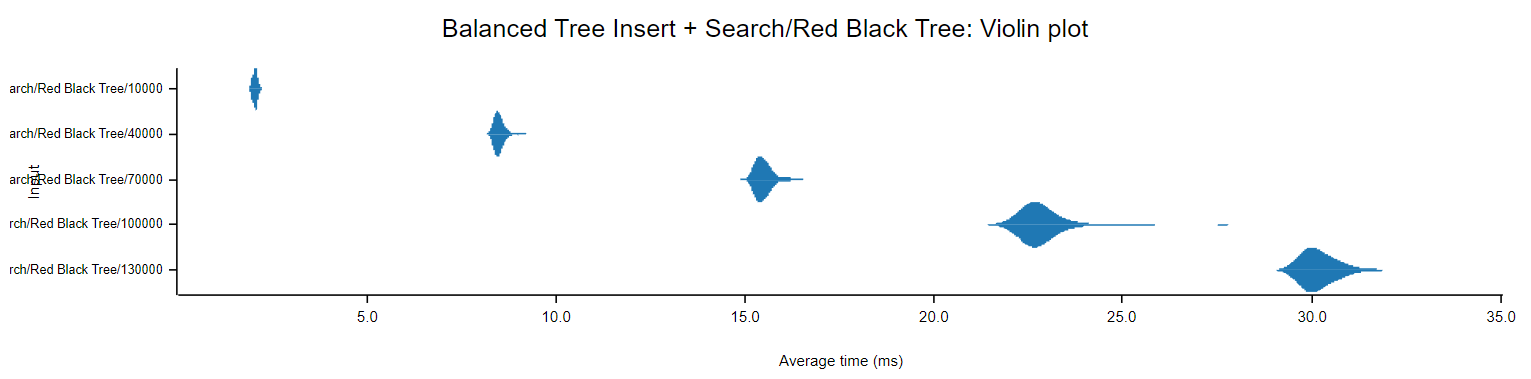
\includegraphics[width=15cm]{benchmarks/Red_black_tree/violin.png}
    \label{Violin}
\end{figure}

The following chart shows the mean measured time for each function as the input (or the size of the input) increases. \\

\begin{figure}[htbp]
    \centering
    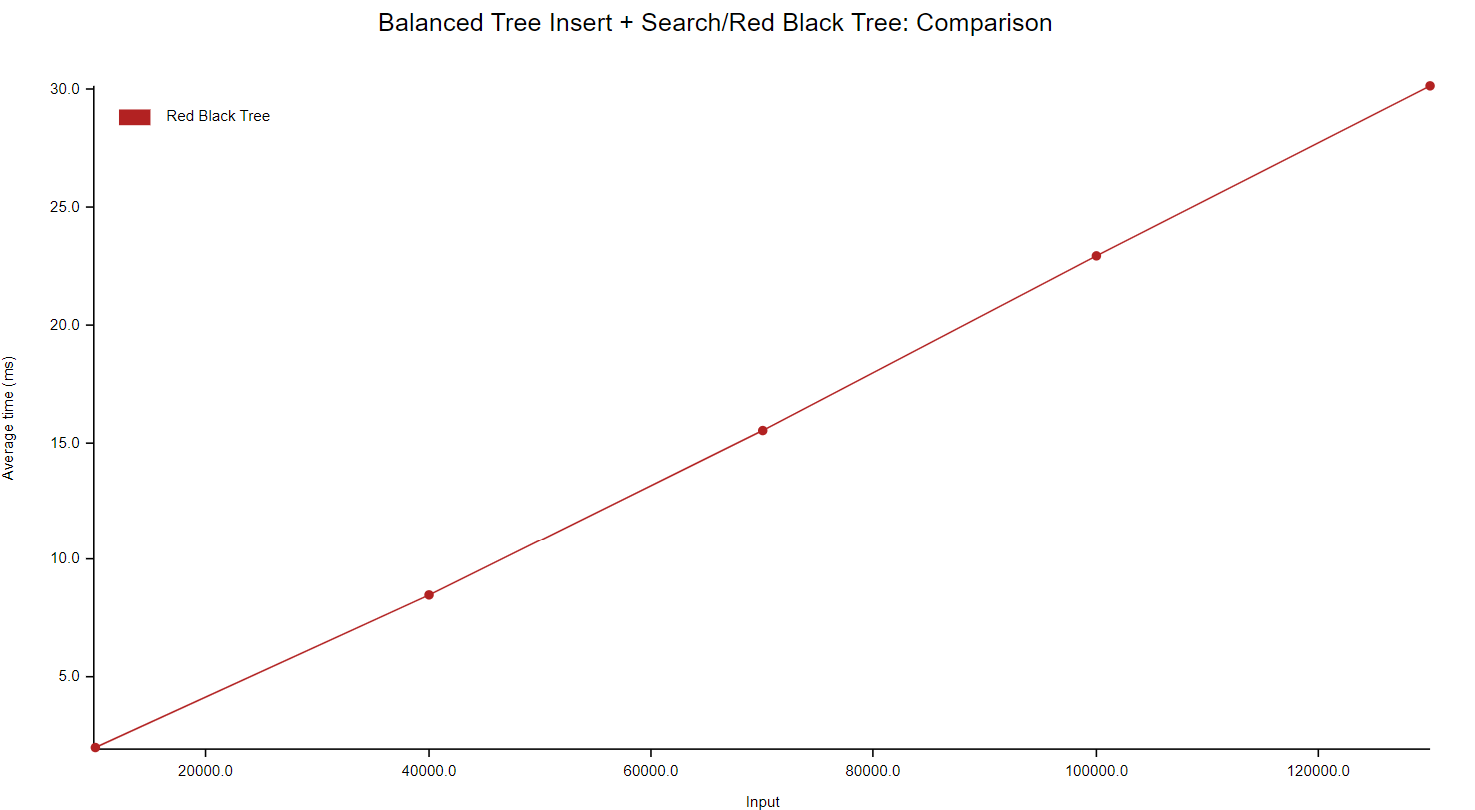
\includegraphics[width=8cm]{benchmarks/Red_black_tree/line.png}
    \label{Line}
\end{figure}

\mintinline{text}{Balanced Tree Insert + Search/Red Black Tree/10000}
\columnratio{0.75}
\begin{paracol}{3}
    \centering        
    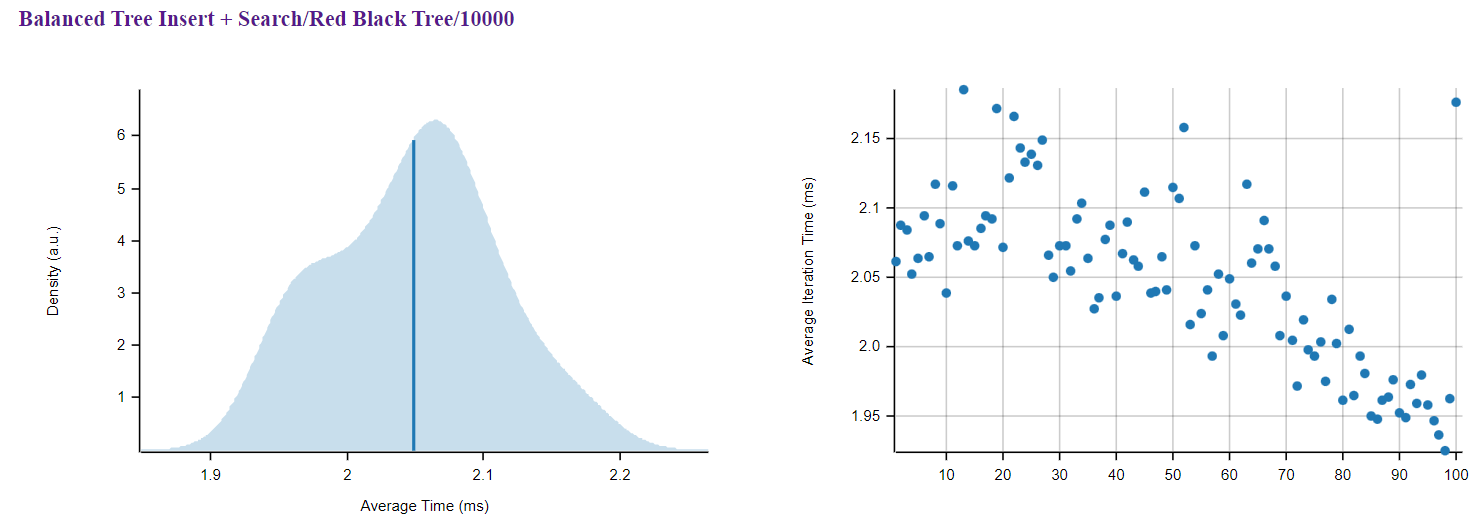
\includegraphics[width=11cm]{benchmarks/Red_black_tree/10000/plots.png}
    \switchcolumn
    \vspace*{\fill}
    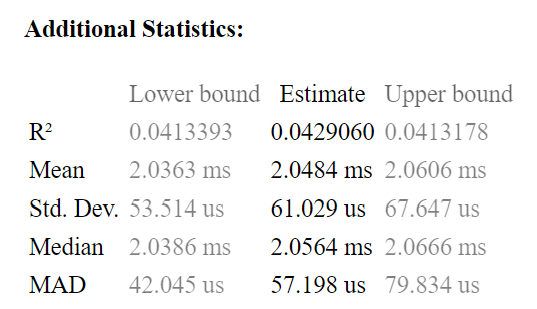
\includegraphics[width=4cm]{benchmarks/Red_black_tree/10000/stats.png}
    \vspace*{\fill}
\end{paracol}

\mintinline{text}{Balanced Tree Insert + Search/Red Black Tree/40000}
\columnratio{0.75}
\begin{paracol}{3}
    \centering        
    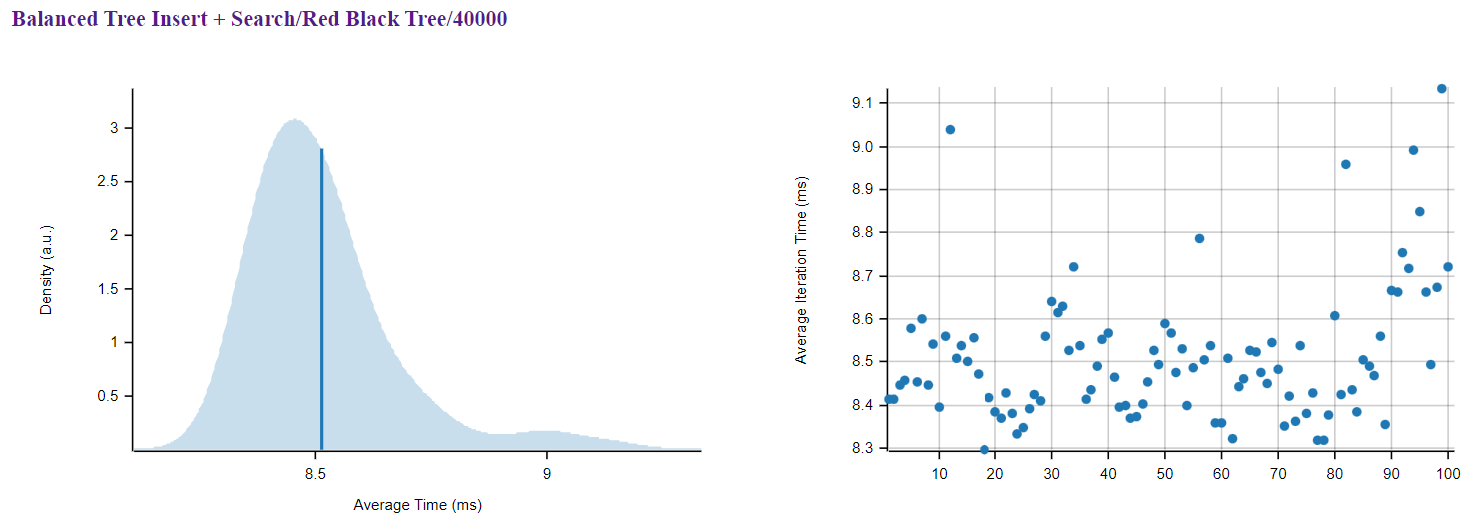
\includegraphics[width=11cm]{benchmarks/Red_black_tree/40000/plots.png}
    \switchcolumn
    \vspace*{\fill}
    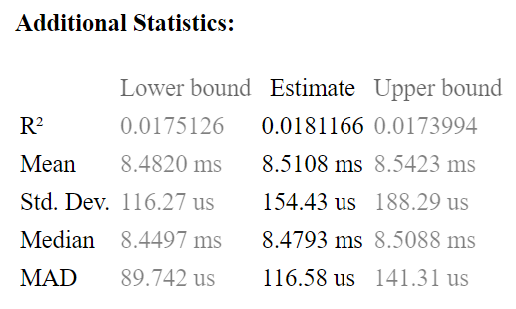
\includegraphics[width=4cm]{benchmarks/Red_black_tree/40000/stats.png}
    \vspace*{\fill}
\end{paracol}

\mintinline{text}{Balanced Tree Insert + Search/Red Black Tree/70000}
\columnratio{0.75}
\begin{paracol}{3}
    \centering        
    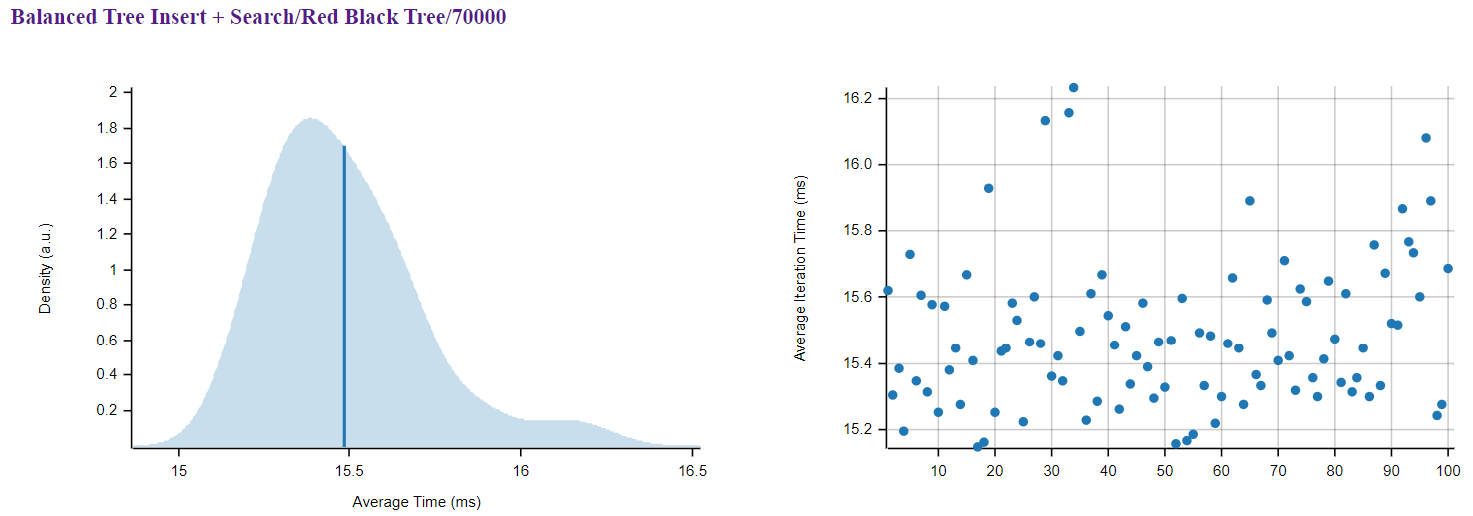
\includegraphics[width=11cm]{benchmarks/Red_black_tree/70000/plots.png}
    \switchcolumn
    \vspace*{\fill}
    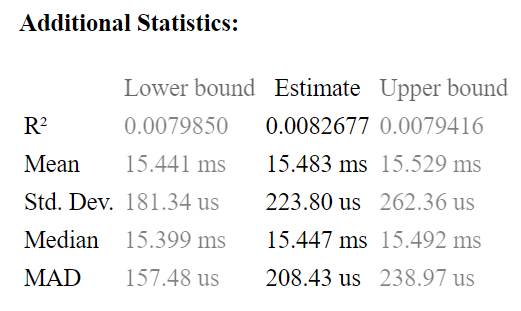
\includegraphics[width=4cm]{benchmarks/Red_black_tree/70000/stats.png}
    \vspace*{\fill}
\end{paracol}

\newpage
\mintinline{text}{Balanced Tree Insert + Search/Red Black Tree/100000}
\columnratio{0.75}
\begin{paracol}{3}
    \centering        
    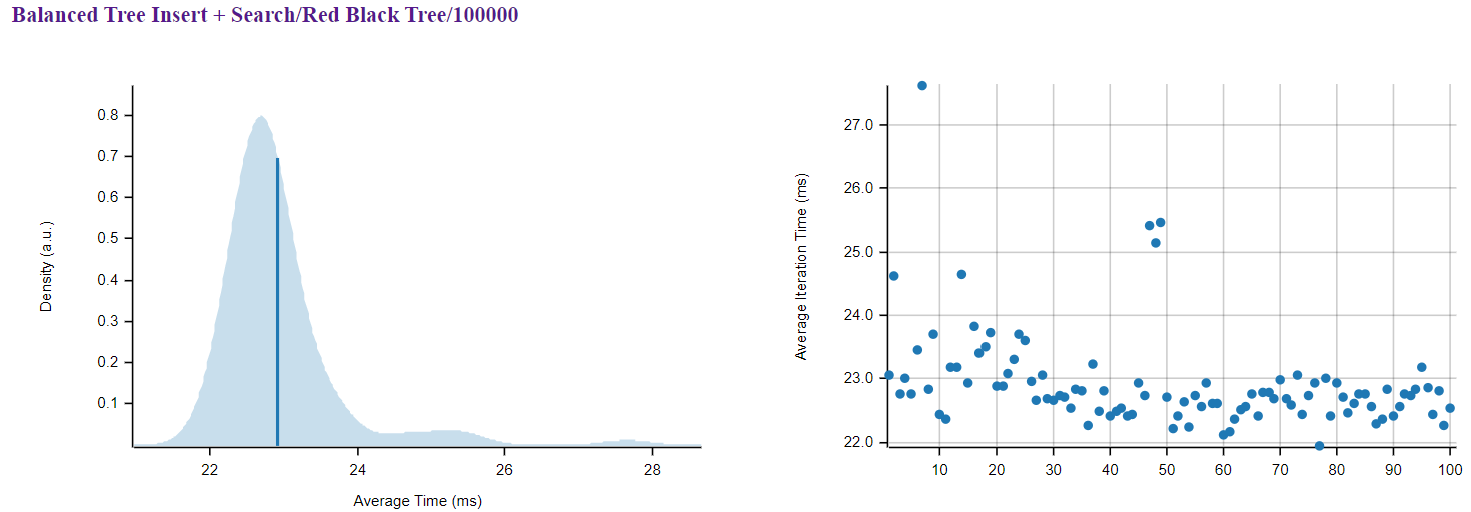
\includegraphics[width=11cm]{benchmarks/Red_black_tree/100000/plots.png}
    \switchcolumn
    \vspace*{\fill}
    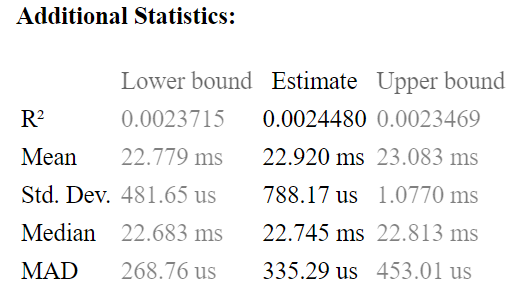
\includegraphics[width=4cm]{benchmarks/Red_black_tree/100000/stats.png}
    \vspace*{\fill}
\end{paracol}

\mintinline{text}{Balanced Tree Insert + Search/Red Black Tree/130000}
\columnratio{0.75}
\begin{paracol}{3}
    \centering        
    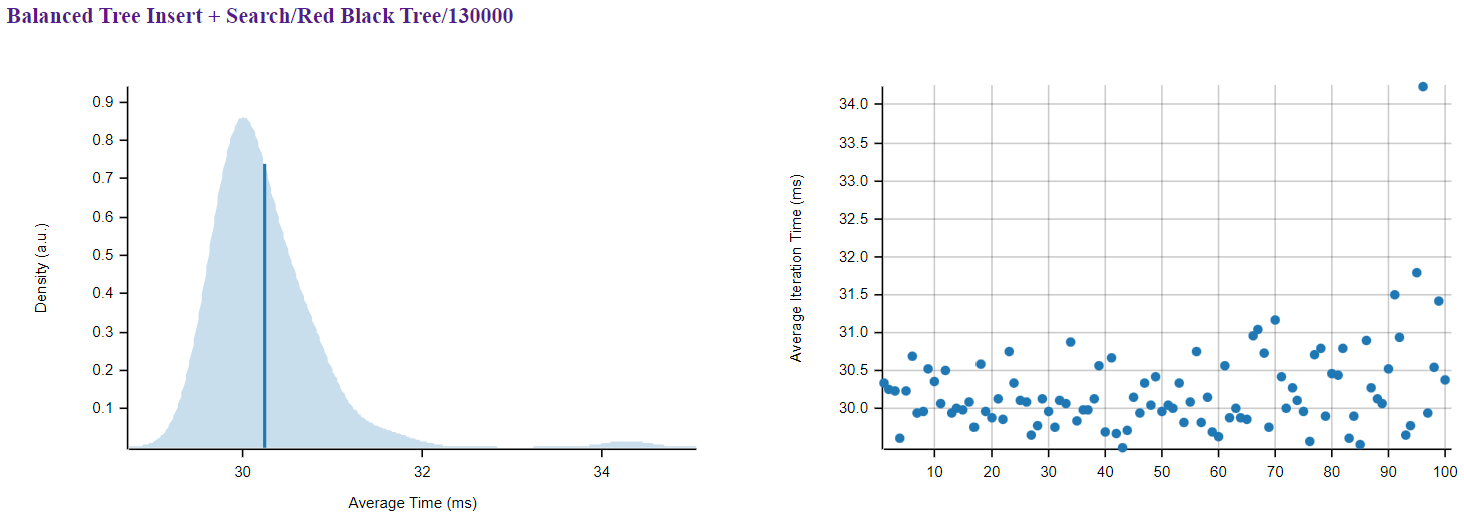
\includegraphics[width=11cm]{benchmarks/Red_black_tree/130000/plots.png}
    \switchcolumn
    \vspace*{\fill}
    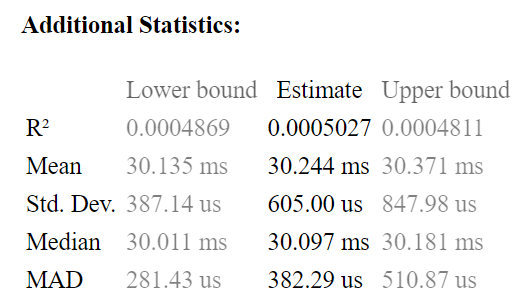
\includegraphics[width=4cm]{benchmarks/Red_black_tree/130000/stats.png}
    \vspace*{\fill}
\end{paracol}
\newpage
\subsection{AVL Tree}
The following chart shows the relationship between function/parameter and iteration time. The thickness of the shaded region indicates the probability that a measurement of the given function/parameter would take a particular length of time.
\begin{figure}[htbp]
    \centering
    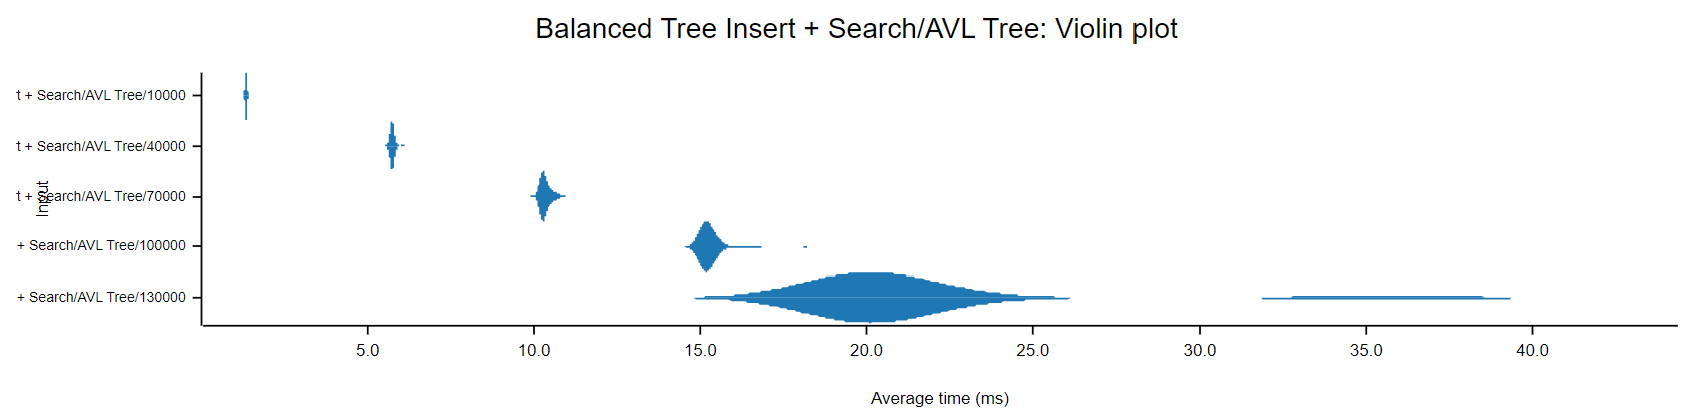
\includegraphics[width=15cm]{benchmarks/AVL/violin.png}
    \label{Violin_AVL}
\end{figure}

The following chart shows the mean measured time for each function as the input (or the size of the input) increases. \\

\begin{figure}[htbp]
    \centering
    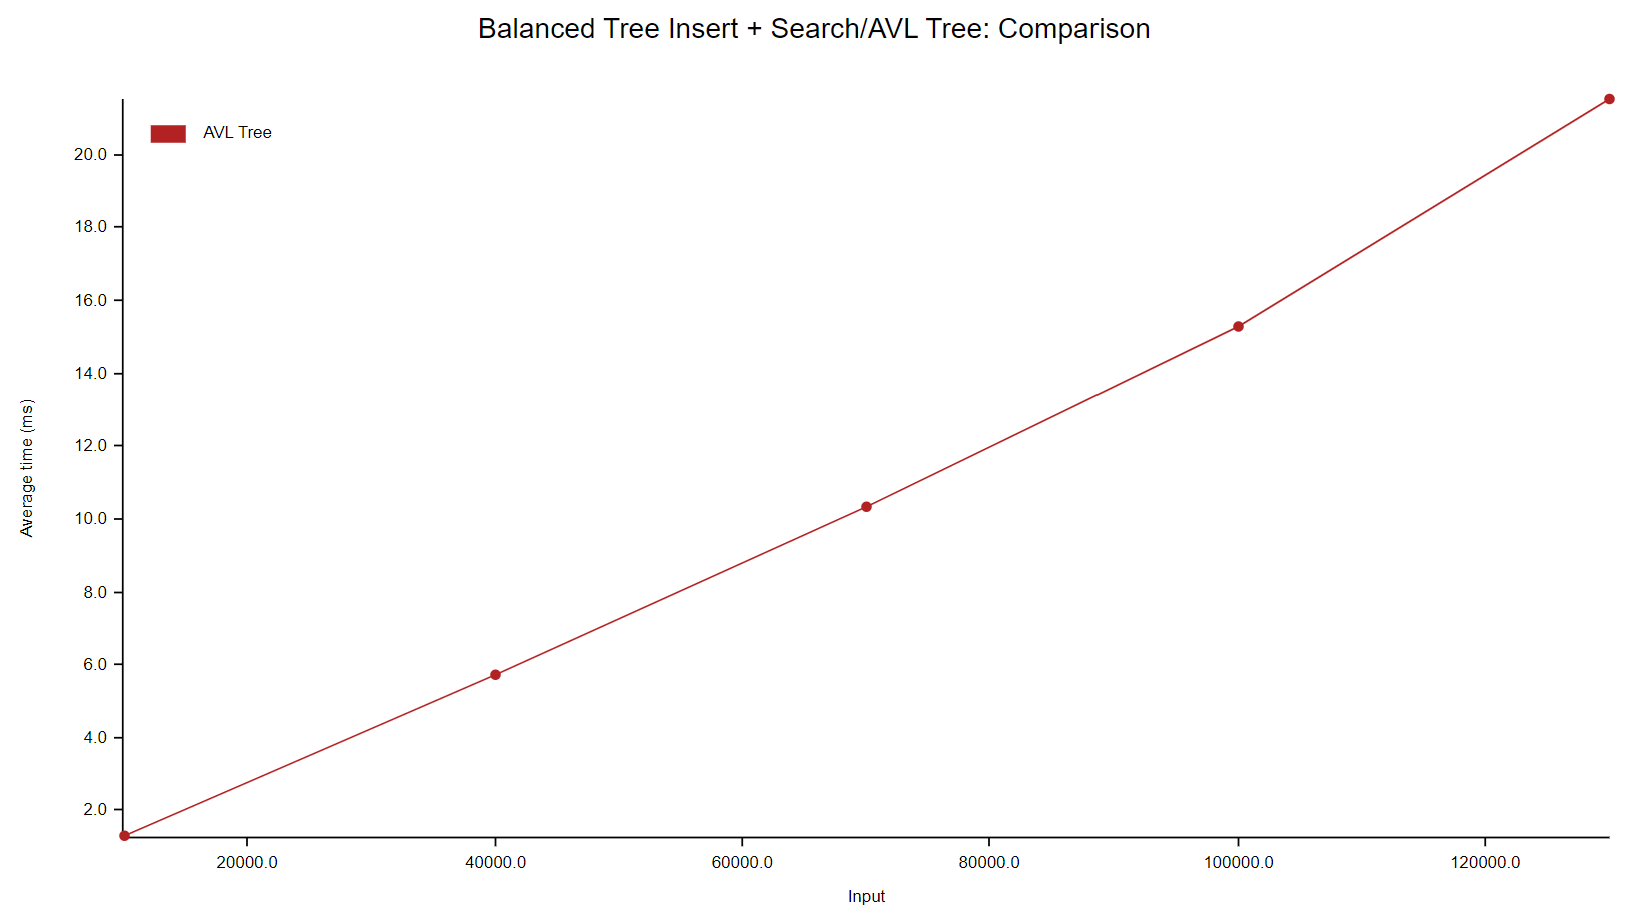
\includegraphics[width=8cm]{benchmarks/AVL/line.png}
    \label{Line_AVL}
\end{figure}
\newpage
\mintinline{text}{Balanced Tree Insert + Search/AVL Tree/10000}
\columnratio{0.75}
\begin{paracol}{3}
    \centering        
    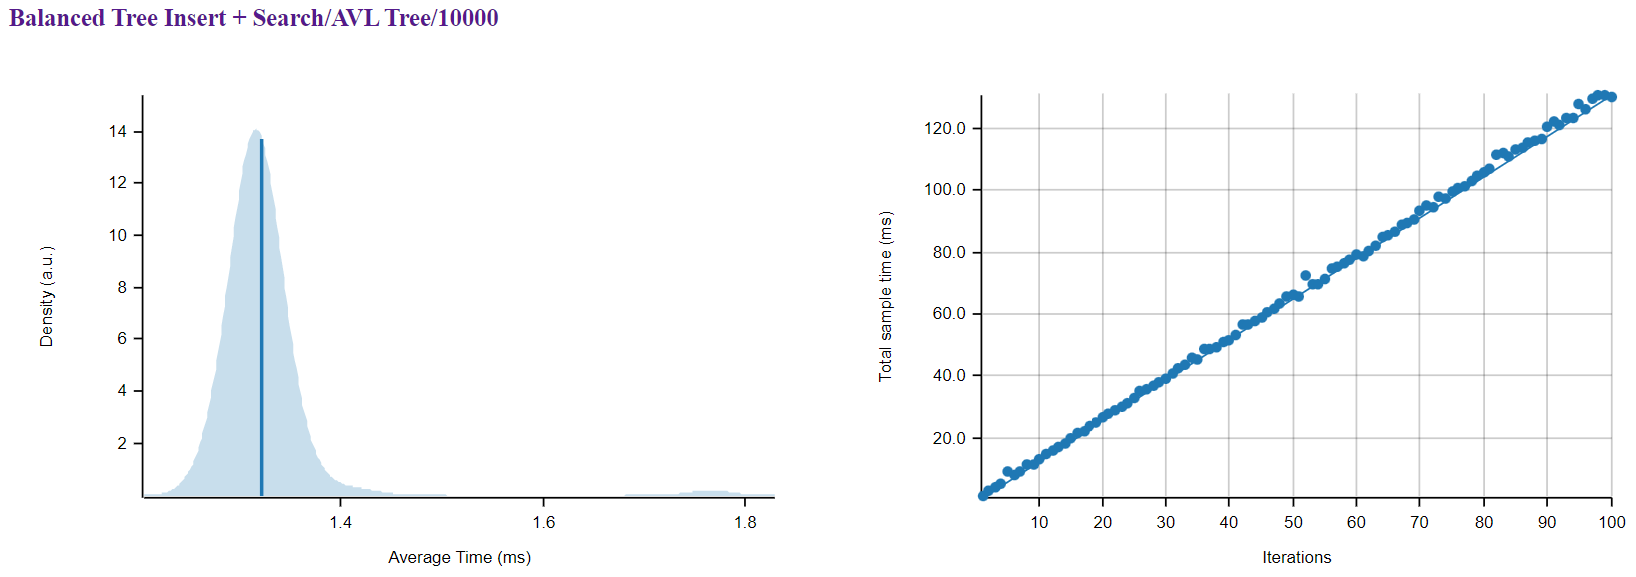
\includegraphics[width=11cm]{benchmarks/AVL/10000/plots.png}
    \switchcolumn
    \vspace*{\fill}
    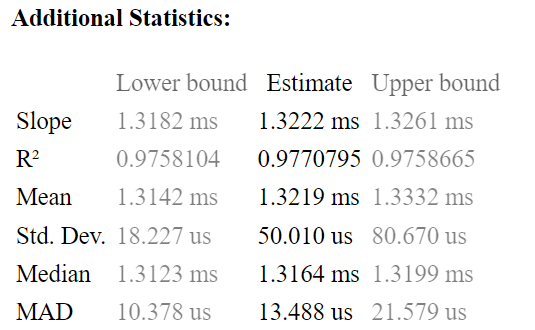
\includegraphics[width=4cm]{benchmarks/AVL/10000/stats.png}
    \vspace*{\fill}
\end{paracol}

\mintinline{text}{Balanced Tree Insert + Search/AVL Tree/40000}
\columnratio{0.75}
\begin{paracol}{3}
    \centering        
    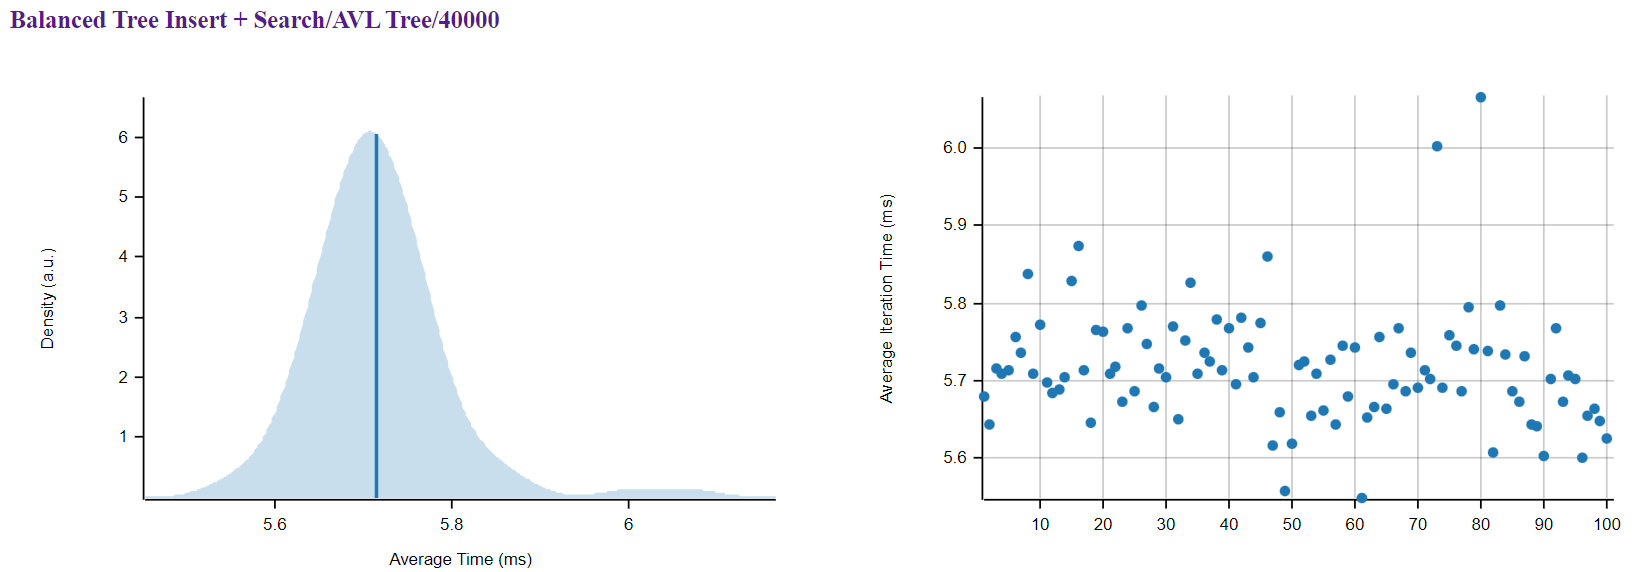
\includegraphics[width=11cm]{benchmarks/AVL/40000/plots.png}
    \switchcolumn
    \vspace*{\fill}
    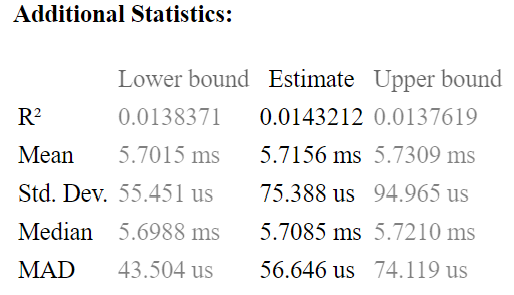
\includegraphics[width=4cm]{benchmarks/AVL/40000/stats.png}
    \vspace*{\fill}
\end{paracol}

\mintinline{text}{Balanced Tree Insert + Search/AVL Tree/70000}
\columnratio{0.75}
\begin{paracol}{3}
    \centering        
    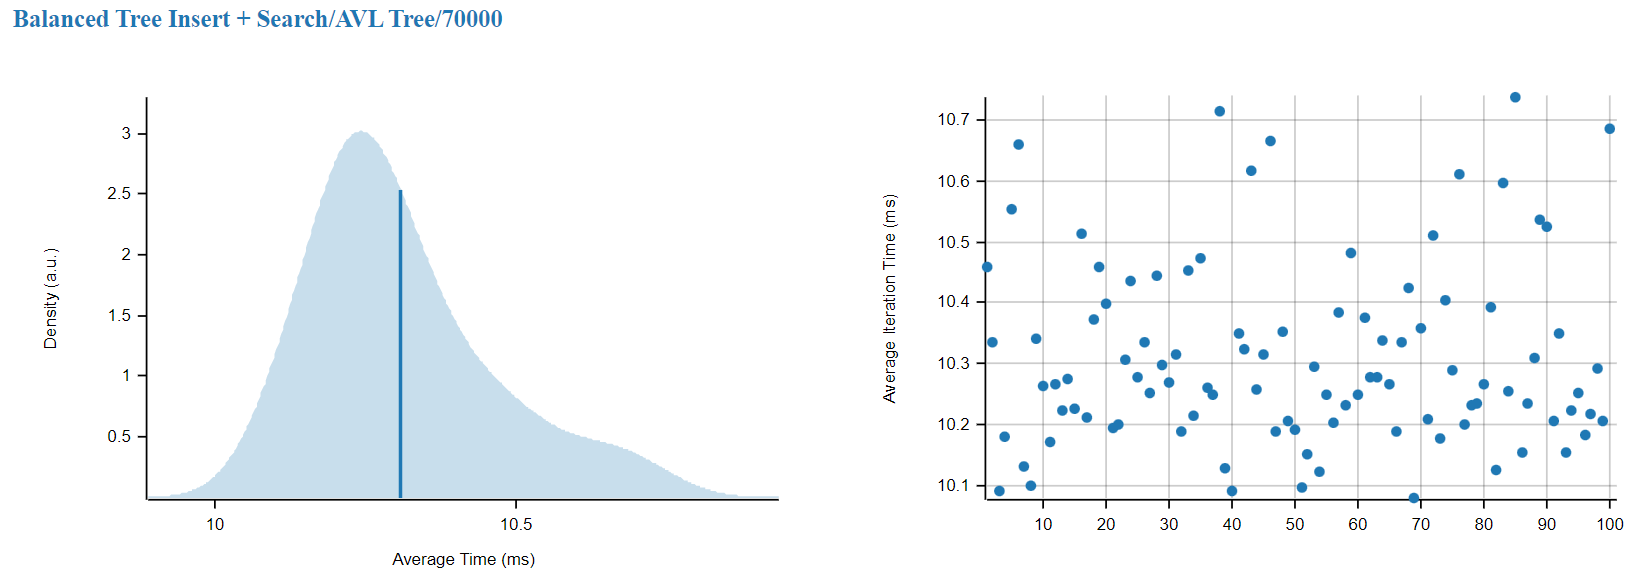
\includegraphics[width=11cm]{benchmarks/AVL/70000/plots.png}
    \switchcolumn
    \vspace*{\fill}
    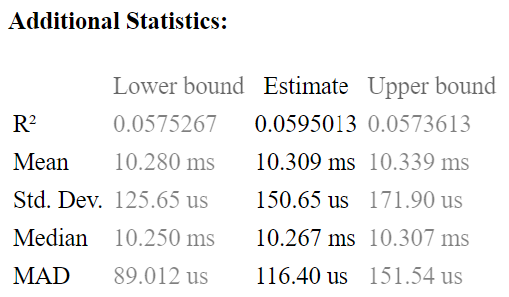
\includegraphics[width=4cm]{benchmarks/AVL/70000/stats.png}
    \vspace*{\fill}
\end{paracol}

\newpage
\mintinline{text}{Balanced Tree Insert + Search/AVL Tree/100000}
\columnratio{0.75}
\begin{paracol}{3}
    \centering        
    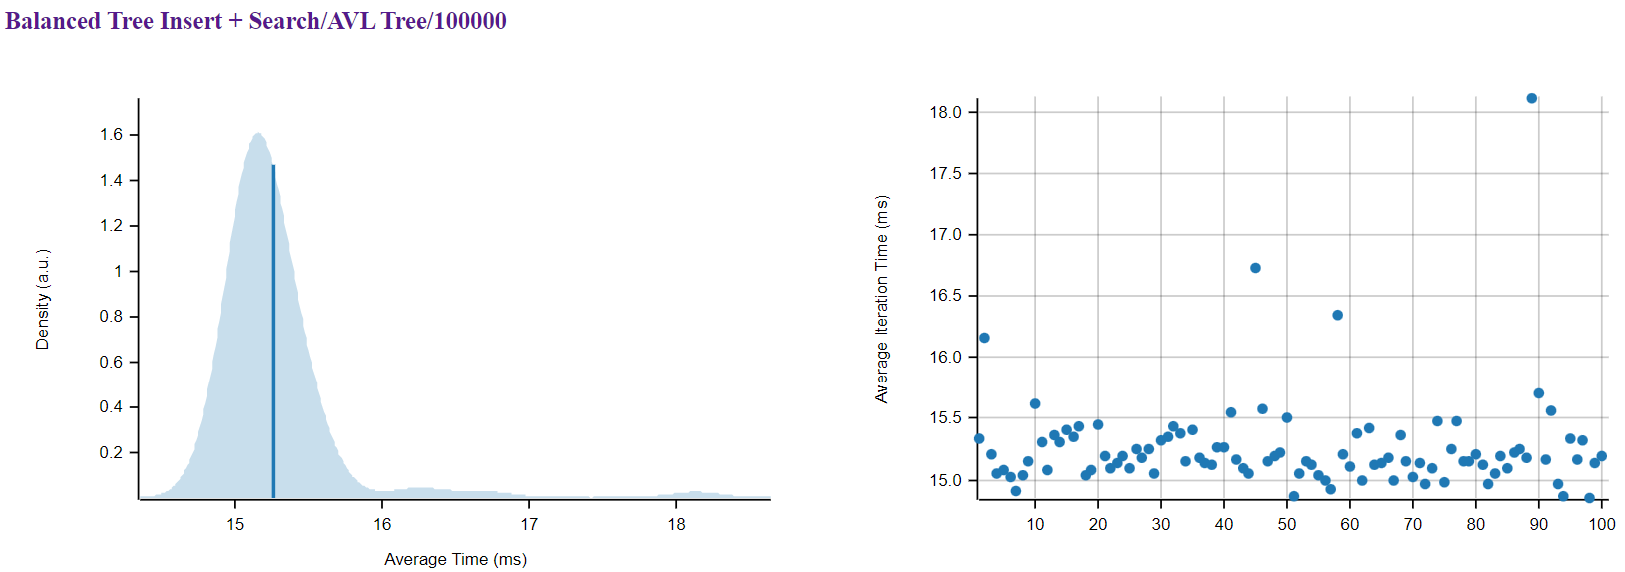
\includegraphics[width=11cm]{benchmarks/AVL/100000/plots.png}
    \switchcolumn
    \vspace*{\fill}
    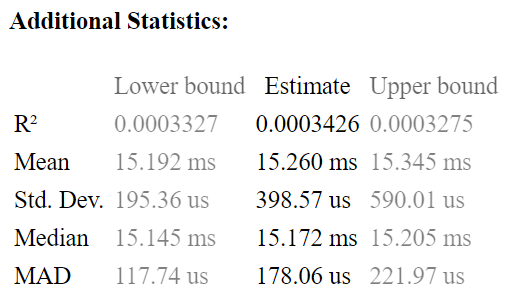
\includegraphics[width=4cm]{benchmarks/AVL/100000/stats.png}
    \vspace*{\fill}
\end{paracol}

\mintinline{text}{Balanced Tree Insert + Search/AVL Tree/130000}
\columnratio{0.75}
\begin{paracol}{3}
    \centering        
    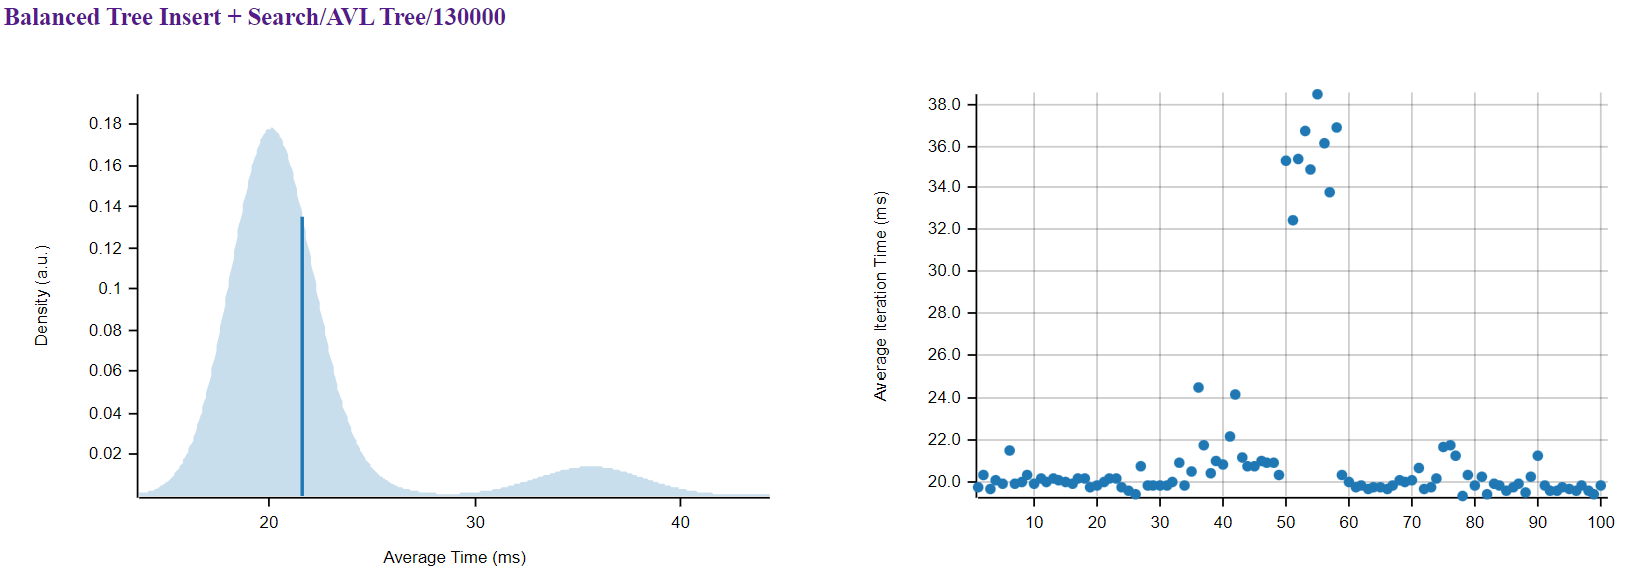
\includegraphics[width=11cm]{benchmarks/AVL/130000/plots.png}
    \switchcolumn
    \vspace*{\fill}
    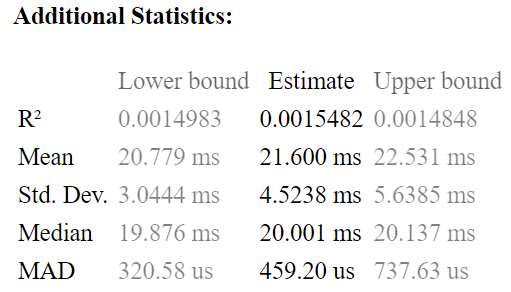
\includegraphics[width=4cm]{benchmarks/AVL/130000/stats.png}
    \vspace*{\fill}
\end{paracol}

\subsection{Comparison}
For every case the AVL Tree performs noticeably better than the Red Black Tree illustrating that the AVL Tree is more efficient.
However, this conclusion really can only be said for this worst possible ``insert and search" case.  This does not provide insight on best case behavior or on random behavior.
Furthermore we have no benchmarks for any deletion case.  These additional benchmarks would be valuable data for getting a more complete picture on how
the two data structures differ performance wise.  As well, if we have any knowledge of the data we expect to receive we can use the additional bookmarks to select the best data structure for the
case we are most likely to match.

Using a binary search tree as a baseline measurement is not likely to be necessary.  We know that the worst case complexity of the AVL Tree and Red Black Tree are better than
that of a binary search tree and the comparison is between the two trees.  However if we include more benchmarks for other cases having a baseline might be more beneficial
so we may get a better picture of how more general cases actually compare.  It might also be beneficial to include benchmarks for 2-3-4 Trees and B-Trees.  Again, this way we can get
more information regarding what sort of tree would be the best fit for our use case (provided we know anything in advance about how the tree will get used most commonly).

\pagebreak

\section{User Manual}

\subsection{Tree}
The  \mintinline{text}{Tree T, U} type represents a binary search tree to search  \mintinline{text}{T} and is balanced by \mintinline{text}{U}.
The following are methods of the public interface for manipulating a \mintinline{text}{Tree} instance:
\begin{itemize}
    \item \mintinline{text}{Tree::new} - constructs an empty tree
    \item \mintinline{text}{Tree::is_empty} - returns true if the tree has no nodes
    \item \mintinline{text}{Tree::insert} - inserts a key, rebalancing using  \mintinline{text}{U}
    \item \mintinline{text}{Tree::search} - returns true if the key was found in the tree
    \item \mintinline{text}{Tree::delete} - removes and returns a key, rebalancing using  \mintinline{text}{U}
    \item \mintinline{text}{Tree::height} - returns the height of the tree
    \item \mintinline{text}{Tree:leaves} - returns the number of leaf nodes in the tree   
\end{itemize}

\subsection{Pre-Defined Types}
The following are other predefined types for basic \mintinline{text}{Tree} usage
\begin{itemize}
    \item \mintinline{text}{avl::AVLBalance} - \mintinline{text}{TreeBalance} type using AVL Tree rules
    \item \mintinline{text}{AVLTree} - typedef for tree that uses AVLBalance
    \item \mintinline{text}{redblack::RedBlackTree} - \mintinline{text}{TreeBalance} type using Red Black Tree rules
    \item \mintinline{text}{RedBlackTree} - typedef for tree that uses  \mintinline{text}{RedBlackBalance}
    \item \mintinline{text}{BinarySearchTree} - typedef for a tree that doesn't perform any balancing
\end{itemize}

\subsection{TreeBalance Trait Implementation}
The \mintinline{text}{TreeBalance} trait can be used to perform rebalancing on a tree using custom rules.
A type that implements the trait and is associated with a \mintinline{text}{Tree} instance will have the trait functions called
to perform rebalancing.  Review \mintinline{text}{TreeBalance} and relevant type documentation for more information as we will not
describe it further here.

\subsection{CLI Demo}
We have built a CLI that allows users to test both the Red Black Tree and the AVL Tree. Upon starting the program (located in \mintinline{text}{main.rs}), the user will be greeted by a welcome message. The user will also be prompted to select which type of tree they would like to test. In order to test a Red Black Tree, the user needs to enter `1'; to test an AVL Tree, the user needs to enter `2'. 

Upon selecting a tree, the user will be presented with a list of commands. Here is a summary of the commands available:
\begin{itemize}
    \item \mintinline{text}{insert <n>}     - insert \mintinline{text}{<n>} into the tree
    \item \mintinline{text}{delete <n>}     - delete \mintinline{text}{<n>} from the tree
    \item \mintinline{text}{search <n>}     - output whether \mintinline{text}{<n>} is in the tree or not
    \item \mintinline{text}{clear}          - clear all elements from the tree
    \item \mintinline{text}{isempty}        - output whether the tree is empty or not
    \item \mintinline{text}{height}         - output the height of the tree
    \item \mintinline{text}{leaves}         - output the number of leaves in the tree
    \item \mintinline{text}{print tree}     - print formatted tree
    \item \mintinline{text}{print inorder}  - print elements using inorder traversal
    \item \mintinline{text}{switch}         - select a new tree type
    \item \mintinline{text}{help}           - reprint this menu
    \item \mintinline{text}{exit}           - exit program
\end{itemize}

For example, let's say we want to select an AVL Tree and insert 3, 5, and 2 into the tree. We would first enter `2' followed by \mintinline{text}{insert 3}, \mintinline{text}{insert 5}, and \mintinline{text}{insert 2}.

\end{document}